\documentclass{grattanAlpha}

\title{Report}
\author{author}

\addbibresource{AP-bibliography.bib}

\begin{document}
\contentspage

\begin{overview}[-40pt]
A federal election is an opportunity to take stock of how Australia
is doing, where it’s going, and what governments can do about it.
This report surveys policy recommendations from seven years of
Grattan Institute reports and outlines what the Commonwealth
Government should do to improve Australia.

The problems aren’t hard to find. Per capita national income has
fallen over the last four years as the mining boom subsided.
Economic growth is slow, reflecting trends across the developed
world. Unemployment stands at nearly six per cent, higher than in
the United States and United Kingdom, countries hit much harder
by the Global Financial Crisis than Australia. Underemployment
also remains high.

Commonwealth budgets haven’t come close to balancing for eight
years. Interest on the accumulating debt now consumes 4 per
cent of government income, or as much as the Commonwealth
spends on public hospitals. Younger generations will be taxed
more to pay for today’s spending. Every \$40 billion deficit, the
norm for each of the last eight years, forces households aged 25
to 34 to pay an extra \$10,000 in tax over their working lives.
Our large capital cities have growing pains. House prices are very
high relative to incomes. Home ownership is falling for all
households aged under 55. Most new housing is far from the city
centres where most new jobs are being created. More people
spend longer in traffic getting to work. The physical divide
between rich and poor is growing.

School education is not keeping up with the best in the world. Test
results are well behind international benchmarks, and Australia is
slipping down global rankings. Between Years Three and Nine,
talented students from poorer backgrounds fall almost two years
behind their peers from richer backgrounds.

Our political system is not dealing well with these challenges.
Politicians are often creating great expectations that far exceed
what government can ever do. Meanwhile, they are failing to act
on the things that they can control. The result is an often barren
debate that disappoints everyone and makes for a dull campaign.
Yet there are many reforms that can contribute to economic
growth, improve the quality and reduce the cost of government
services, and bring budgets back into balance. A growing
evidence base shows which reforms would work.

Progress on this agenda has been underwhelming for a decade,
perhaps because the prosperity of the mining boom sapped the
will for reform. The politics of reform is never easy. Vested interest
groups, emboldened by success, are more vocal in protecting
their interests. Meanwhile the public interest has few friends.
Ironically, though, the public seems to be up for reform. Surveys
suggest that people understand the need for budget repair, and
are even prepared to contemplate slaying sacred cows such as
negative gearing.

Our politics can implement this reform agenda by using the
evidence that has been assembled, robustly articulating the public
interest, and staring down interest groups. Australia has a proud
history of enlightened public policy. Many countries would be
delighted to swap our problems for theirs. Australia can continue
to be the lucky country. But we must make our own luck.
\end{overview}

\chapter{Economic growth priorities}
\begin{verysmallbox}[H]{Summary}{box:economic-growth-priorities}
Improving the efficiency of Australian taxes could provide a big
kick to economic growth. In particular, the Commonwealth should
encourage the States to replace stamp duties by general property
taxes.

Lifting workforce participation rates for women and older workers
could boost economic growth, and counter the ageing of the
workforce. The Commonwealth should ask the Productivity
Commission to assess combinations of tax, transfer, and
childcare support that would reduce welfare traps and encourage
higher female labour force participation for a given budgetary
cost. The Commonwealth should also raise the age of access to
the Age Pension and superannuation to 70 years.

Government should remove inappropriate impediments to
flexibility in the economy, so that resources can be swiftly
reallocated to their highest value uses as conditions change.
Government should remove barriers to innovation, but should not
waste money in its name. Removing barriers to the local spread of
global innovations is likely to make more difference to economic
growth than subsidies for Australian inventions.

With many of the economy-wide reforms already completed,
industry-specific reforms – especially in sectors such as
superannuation – may well comprise the bulk of the productivity
increases that government reform can achieve.
\end{verysmallbox}

\section{Scope}
This report aims to help the next Commonwealth Government to
set priorities for reform. Drawing primarily on work published by
Grattan Institute over the last seven years, it identifies policy
changes that the Government should adopt to make the most
difference to the lives of Australians.

The report considers reforms to increase economic growth and
reduce budget deficits. It discusses reforms to policy for tax and
budgets, cities, transport, energy, school education, higher
education and health. Grattan Institute has focused on these
because they make a big difference to the lives of Australians,
because analysis can chart a path to better policy, and because
outcomes are too often driven by vested interests rather than the
public interest.

The report does not cover areas such as foreign affairs and trade,
immigration, defence and security, law and order, industrial
relations, communications, human services, indigenous affairs
and the environment. These areas matter, but have not been part
of Grattan Institute’s work to date.

The report focuses on issues that the Commonwealth can
influence directly rather than those that are essentially State
responsibilities. It selectively identifies areas where there might be
a clear rationale for the Commonwealth to make additional tied
grants to the States.\footnote{In this report, “States and Territories” are abbreviated to “States”.} 
These areas include situations where the Commonwealth budget would substantially benefit from State
Government reforms.


\section{Spending projections}
The Commonwealth’s spending projections also seem optimistic. They assume tight spending restraint, with government spending falling as a share of the economy (\Cref{fig:FISCAL-2}).\footcite[][5--11]{Treasury2015BudgetPapers201516}  The projections forecast spending to grow at just 2.6~per cent a year on average between 2014\nobreakdash-15 and 2025\nobreakdash-26, far below the 3.6~per~cent average growth rate of the last decade.\footcite[][5]{PBO2015}  Consistent with this spending restraint, the Commonwealth Government forecasts that spending will decline to 24.2 per cent of GDP in 2024-25, below its long term average.\footcite[][3--9]{Treasury2015BudgetPapers201516}  

Spending is forecast to be below the historical average in all program areas other than defence, as is shown in \Vref{fig:FISCAL-8}, which compares the projected growth in the Commonwealth’s largest spending programs over the next 10 years with the history of the last 10~years. 

\begin{figure}
\caption{Spending forecasts rely on lower growth in almost all major programme areas\label{fig:FISCAL-8}}%
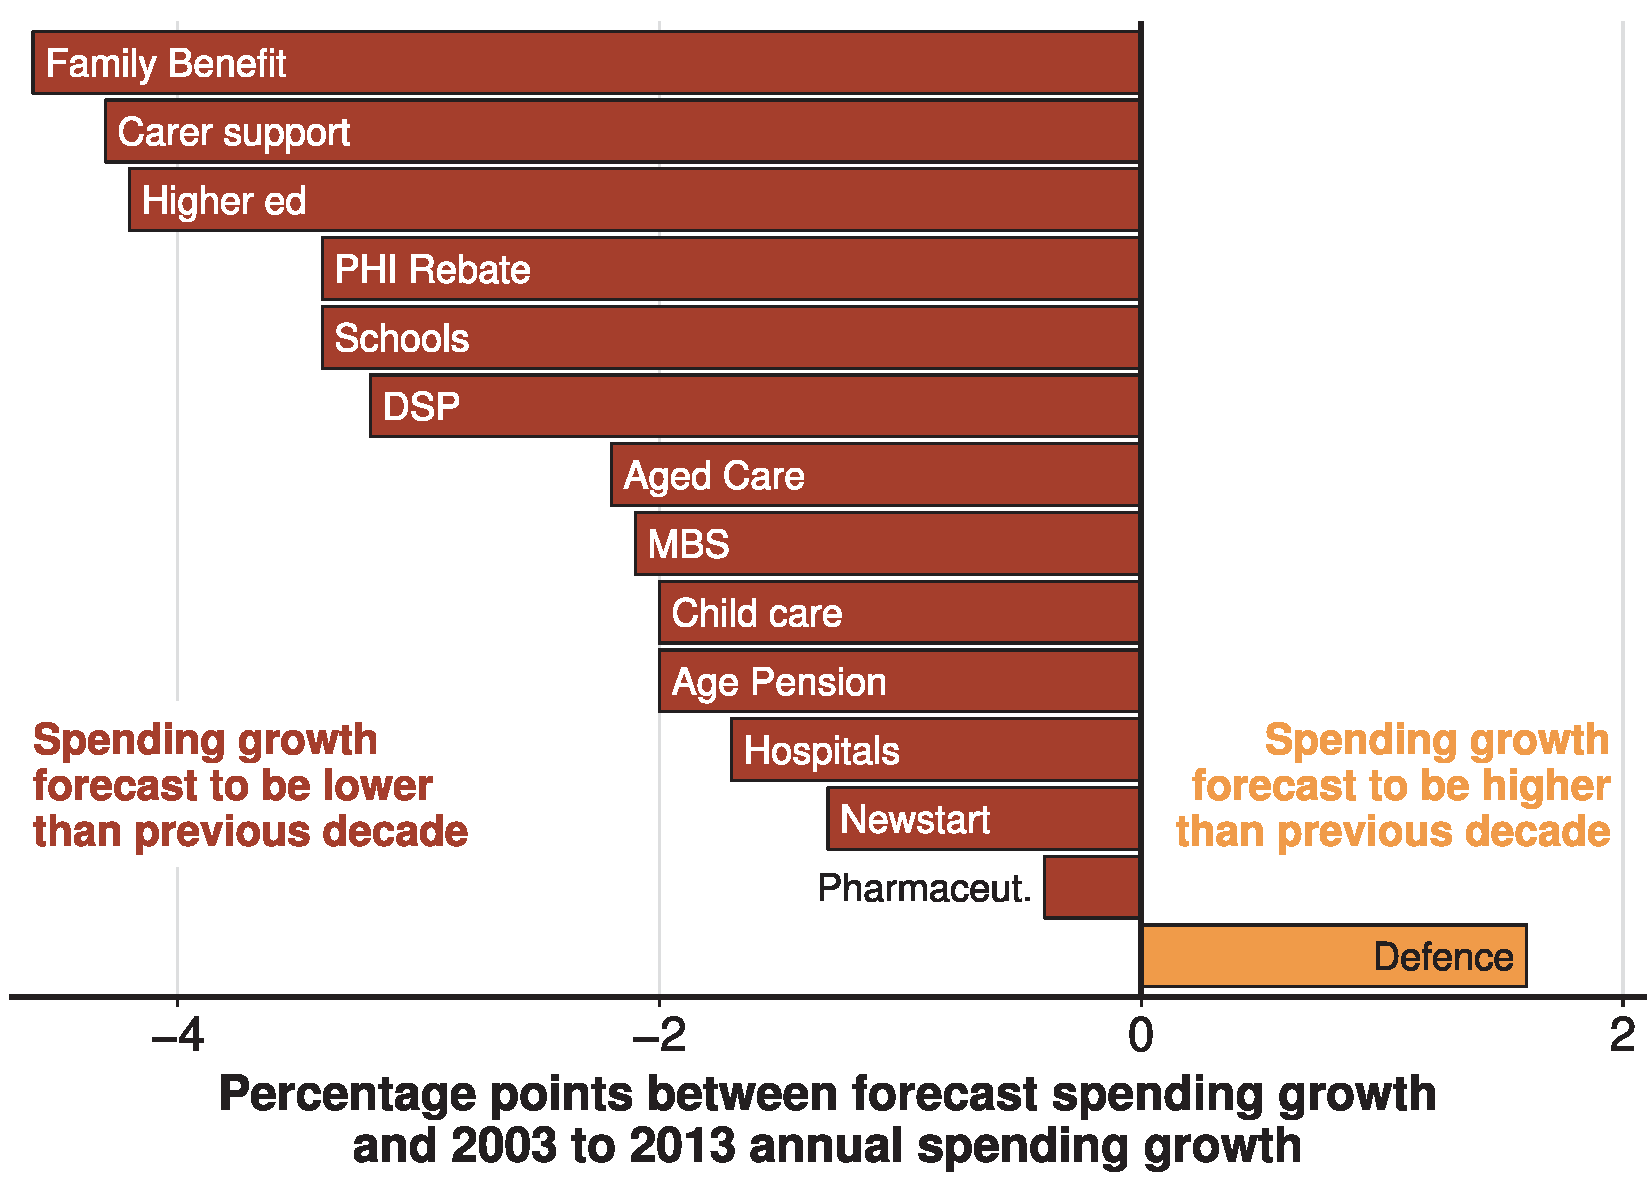
\includegraphics[width=\columnwidth]{figure/budget-repair-Figure8-altered-1.pdf}
\noteswithsource{The defence estimates do not factor in the commitment to increase defence spending to 2~per~cent of GDP by 2023-24. Rather they are based on the long-term funding commitments made in previous Defence White Papers and government announcements.}{{\textcite{PBO2014}}}
\end{figure}

Some of these estimates seem improbable. For example, it seems unlikely that spending on demand-driven programs such as the \textbf{Medicare Benefits Schedule} will moderate without significant policy changes. The PBO attributes the strong historical growth in Medicare payments to policies (such as the Bulk Billing Incentive and the Extended Medicare Safety Net) that have made Medicare services more attractive or accessible. New policy measures such as the freeze in Medicare scheduled fees are forecast to produce lower growth. Yet for more than 20 years the ageing of the population, medical science and technology improvements and rising expectations of the health system have put relentless pressure on the health budget.\footcite{Daley2014}  These pressures will not abate, and the forecasts almost certainly understate them.

The decline in spending growth for hospitals and schools may be credible given the decision in the 2014-15 Budget to limit spending increases to inflation and population growth. This of course does not mean that spending growth will decline in these program areas – merely that the states will have to bear all of the cost of real per capita growth.

The 2015-16 budget assumes even tighter spending growth than have previous budgets. Except for welfare spending, mainly driven by the NDIS, no category is expected to grow materially faster than inflation.\footcite[][BP No.~1, pp.~5--11]{Treasury2015BudgetPapers201516}  

In other programs, lower forecast growth rates are tied to measures from the 2014-15 and 2015-16 Budgets that are unlikely to be passed by the Senate. Therefore spending on the Carers Payment, higher education and Newstart benefits is likely to be more than forecast. Even the forecast growth in defence spending – the only program area where spending is forecast to grow faster than in the last decade – does not put Australia on a path to spend 2~per~cent of GDP on defence by 2023-24 as the Government has promised.\footnote{See: \textcite[][1]{Defence2014}.} 


Spending projections also assume there will be no new spending initiatives promised at elections or in response to natural disasters or community demands for more assistance to the disadvantaged. Experience over the last decade suggests that such spending restraint will be difficult (\Vref{box:FISCAL-1}).

Given all the number of things that need to go right, moderating spending growth to 24.2~per~cent of GDP in 2024-25 seems extremely unlikely without further explicit budget measures to cut expenditure.


\begin{table}
\captionwithunits{Approaches to valuing properties for council rates vary\label{tbl:PROP-1}}%
{Property value bases that can be used to set council rates in each state}
\begin{tabularx}{\columnwidth}{>{\bfseries}lX}
%
\toprule
\textbf{State} & \textbf{Basis for council rates} \\%[0.5\baselineskip]
\midrule
\textbf{NSW} & Unimproved  \\[0.5\baselineskip]
\textbf{QLD} & Unimproved  \\[0.5\baselineskip]
\textbf{VIC} & Either unimproved or capital improved  \\[0.5\baselineskip]
\textbf{WA} & Capital improved  \\[0.5\baselineskip]
\textbf{SA} & Either unimproved or capital improved \\[0.5\baselineskip]
\textbf{TAS} & Either unimproved or capital improved  \\[0.5\baselineskip]
\textbf{NT} & Unimproved  \\[0.5\baselineskip]
\textbf{ACT} & Unimproved  \\%[0.5\baselineskip]
\bottomrule
\end{tabularx}
\noteswithsource{‘Unimproved’ refers to a set of land valuations that capture the value of the land only. ‘Capital improved’ refers to valuations that capture the value of the land and significant capital improvements made to that land, such as buildings.}{%
\mbox{\textcites{productivity2008assessing}{mangioni2014re}{Treasury2014-Interstate-Comparison-Taxes1415}}.}
\end{table}

\end{document}